%!TEX root = ../larxxia.tex

\chapter{Systems of linear equations}
\label{ch:sle}
\minitoc


Linear relationships are commonly identified in science and engineering, and are commonly expressed as linear equations.
One of the reasons is that scientists and engineers can do amazingly powerful algebraic transformations with linear equations.
Such transformations and their practical implications are the subject of this book.

One vital use in science and engineering is in the scientific task of taking scattered experimental data and \idx{inferring} a general algebraic relation between the quantities measured.
In computing science this task is often called `data mining', `knowledge discovery' or even `artificial intelligence'---although  the algebraic relation is then typically discussed as a computational procedure.
But appearing within these tasks is always linear equations to be solved.

\begin{example}[scientific inference] \label{eg:infertemp}
Two colleagues, and American and a European, discuss the weather; in particular, they discuss the temperature.
\begin{aside}
I am sure you can guess where we are going with this example, but let's pretend we do not know.
\end{aside}
The American says ``yesterday the temperature was~\(80^\circ\) but today is much cooler at~\(60^\circ\)''.
The European says, ``that's not what I heard, I heard the temperature was~\(26^\circ\) and today is~\(15^\circ\)''.
(The marginal figure plots these two data points.)
\marginpar{\begin{tikzpicture}[]
\begin{axis}[footnotesize,width=1.15\marginparwidth
    ,xlabel={European},ylabel={American}
    ,xmin=5,xmax=35,ymin=45,ymax=95]
    \addplot+[only marks] coordinates {(26,80) (15,60)};
    \node at (axis cs:20,70) {?};
    \node at (axis cs:10,50) {?};
    \node at (axis cs:30,90) {?};
\end{axis}
\end{tikzpicture}}%
``Hmmmm, we must be using a different temperature scale'', they say.
Being scientists they start to use linear algebra to \emph{infer}, from the two days of temperature data, a general relation between their temperature scales---a relationship valid over a wide range of temperatures (denoted by the question marks in the marginal figure).
Let's assume that, in terms of the European temperature\(~T_E\), the American temperature \(T_A=cT_E+d\) for some constants\(~c\) and\(~d\) they and we aim to find.
The two days of data then give that
\begin{equation*}
80=c26+d\quad\text{and}\quad 60=c15+d\,.
\end{equation*}
To find\(~c\) and\(~d\):
\begin{itemize}
\item subtract the second equation from the first to deduce \(80-26=26c+d-15c-d\) which simplifies to \(20=11c\), that is, \(c=20/11=1.82\) to two decimal places \twodp;
\item use this value of\(~c\) in either equation, say the second, gives \(60=\frac{20}{11}15+d\) which rearranges to \(d=360/11=32.73\)  to two decimal places \twodp.
\end{itemize}
\marginpar{\begin{tikzpicture}[]
\begin{axis}[footnotesize,width=1.15\marginparwidth
    ,xlabel={European, $T_E$},ylabel={American, $T_A$}
    ,xmin=5,xmax=35,ymin=45,ymax=95]
    \addplot+[only marks] coordinates {(26,80) (15,60)};
    \addplot+[blue,domain=5:35,no marks] {1.82*x+32.73};
\end{axis}
\end{tikzpicture}}%
We deduce that the temperature relationship is \(T_A=1.82\,T_E+32.73\) (as plotted in the marginal figure).
The two colleagues now \emph{predict} that they will be able to use this formula to translate their temperature into that of the other, and vice versa.

You may quite rightly object that the two colleagues \emph{assumed} a linear relation, they do \emph{not know} it is linear.
You may also object that the predicted relation is erroneous as it should be \(T_A=\frac95T_E+32\) (the relation between Celsius and Fahrenheit).
Absolutely, you should object.
Scientifically, the deduced relation  \(T_A=1.82\,T_E+32.73\) is only a conjecture that fits the known data.
More data and more linear algebra together empower us to both confirm the linearity (or not as the case may be), and also to improve the accuracy of the coefficients. 
This is fundamental scientific methodology---and central to it is the algebra of linear equations.
\end{example}


\begin{figure}
\centering
\pgfplotsset{footnotesize,no marks,xlabel={$x$}}
\begin{tabular}{cc}
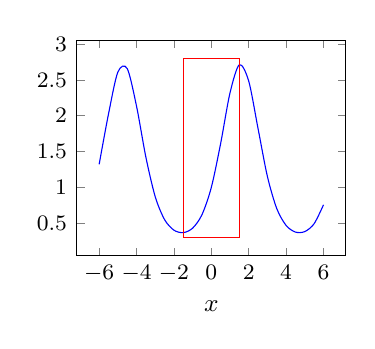
\begin{tikzpicture}[]
\begin{axis}[]
    \addplot+[domain=-6:6,smooth] {exp(sin(deg(x)))};
    \addplot+[] coordinates {
    (-1.5,0.3) (1.5,0.3) (1.5,2.8) (-1.5,2.8) (-1.5,0.3) };
\end{axis}
\end{tikzpicture}
&
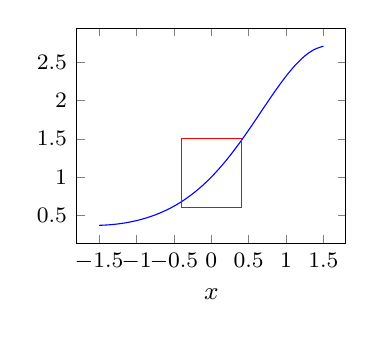
\begin{tikzpicture}[]
\begin{axis}
    \addplot+[domain=-1.5:1.5,smooth] {exp(sin(deg(x)))};
    \addplot+[] coordinates {
    (-0.4,0.6) (0.4,0.6) (0.4,1.5) (-0.4,1.5) (-0.4,0.6) };
\end{axis}
\end{tikzpicture}
\\
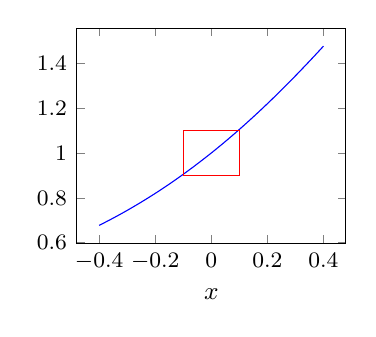
\begin{tikzpicture}[]
\begin{axis}[]
    \addplot+[domain=-0.4:0.4,smooth] {exp(sin(deg(x)))};
    \addplot+[] coordinates {
    (-0.1,0.9) (0.1,0.9) (0.1,1.1) (-0.1,1.1) (-0.1,0.9) };
\end{axis}
\end{tikzpicture}
&
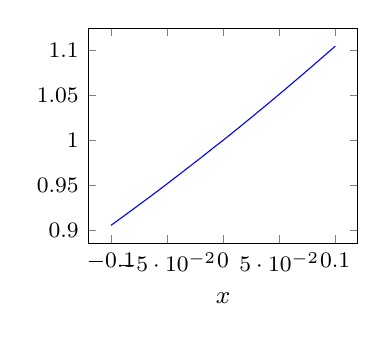
\begin{tikzpicture}[]
\begin{axis}[]
    \addplot+[domain=-0.1:0.1,smooth] {exp(sin(deg(x)))};
\end{axis}
\end{tikzpicture}
\end{tabular}
\caption{zoom in anywhere on any smooth nonlinear curve, such as the plotted~\(f(x)\), and we discover that the curve looks like a straight line on the microscale.
The (red) rectangles show the region plotted in the next graph in the sequence.}
\label{fig:nonlinzoom}
\end{figure}
Linear algebra and equations are also crucial for nonlinear relationships.
Figure~\ref{fig:nonlinzoom} shows four plots of the same nonlinear function, but on successively smaller scales.
Zooming in on the point~\((0,1)\) we see the curve looks straighter and straighter until on the microscale (bottom-right) it is effectively a straight line.
The same is true for everywhere on every smooth nonlinear curve: we discover that every smooth curve looks like a straight line on the microscale. 
Thus we may view any smooth nonlinear function as roughly being made up of lots of microscale straight line segments.
Linear equations and their algebra on this microscale empower our understanding of nonlinear relations---for example, microscale linearity underwrites all of calculus.
 




\endinput





